\chapter{Zero-Knowledge Circuit Implementation}\label{ch:circuit}

This chapter provides a comprehensive analysis of our ZK circuit implementation in Noir. We detail the circuit's input specification, Poseidon hash internals, Merkle tree membership proof, complete code listing with line-by-line analysis, constraint complexity, the UltraHonk proof system, on-chain verifier parameters, and the formal security properties achieved.

\section{Circuit Requirements}

The circuit must prove the following compound statement in zero knowledge:

\begin{quote}
\textit{``I know a secret nullifier $r$ and secret $s$ such that $\Poseidon_2(r, s)$ is a leaf in the Merkle tree with the given root, and $\Poseidon_1(r)$ equals the given nullifier hash, and I am voting for candidate $v$.''}
\end{quote}

This statement simultaneously achieves:
\begin{itemize}
    \item \textbf{Eligibility}: Only registered voters (with commitment in tree) can prove
    \item \textbf{Privacy}: The prover's identity (which leaf) is hidden
    \item \textbf{Uniqueness}: The nullifier hash deterministically identifies the voter for double-vote prevention
    \item \textbf{Vote binding}: The candidate choice is cryptographically bound into the proof
\end{itemize}

\subsection{Input Specification}

\begin{table}[H]
\centering
\caption{Complete circuit input specification with types, visibility, and purpose.}
\label{tab:circuit-inputs}
\begin{tabular}{|l|l|l|l|p{5cm}|}
\hline
\textbf{Name} & \textbf{Type} & \textbf{Visibility} & \textbf{Source} & \textbf{Purpose} \\
\hline
\texttt{nullifier\_hash} & Field & Public & Derived on-device & Double-vote prevention \\
\hline
\texttt{root} & Field & Public & From chain state & Merkle tree root (current) \\
\hline
\texttt{vote} & Field & Public & User selection & Candidate index \\
\hline
\texttt{depth} & u32 & Public & From chain state & Tree depth for path verification \\
\hline
\texttt{nullifier} & Field & Private & Hardware keystore & Secret nullifier (biometric-gated) \\
\hline
\texttt{secret} & Field & Private & Hardware keystore & Secret commitment seed \\
\hline
\texttt{index} & Field & Private & From chain state & Leaf position in tree \\
\hline
\texttt{siblings} & [Field; 16] & Private & From chain state & Merkle authentication path \\
\hline
\end{tabular}
\end{table}

\begin{figure}[H]
\centering
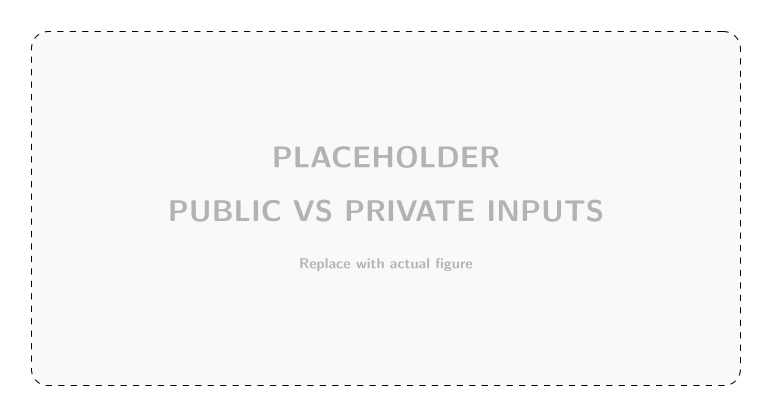
\includegraphics[width=0.85\textwidth]{Images/fig_public_vs_private_inputs.png}
\caption{Public vs. private input separation: public inputs are verified on-chain; private inputs are known only to the prover.}
\label{fig:public-private}
\end{figure}

\section{Poseidon Hash Function Internals}

\subsection{Sponge Construction}

Poseidon uses a sponge construction with state width $t$, rate $r$, and capacity $c = t - r$:

\begin{figure}[H]
\centering
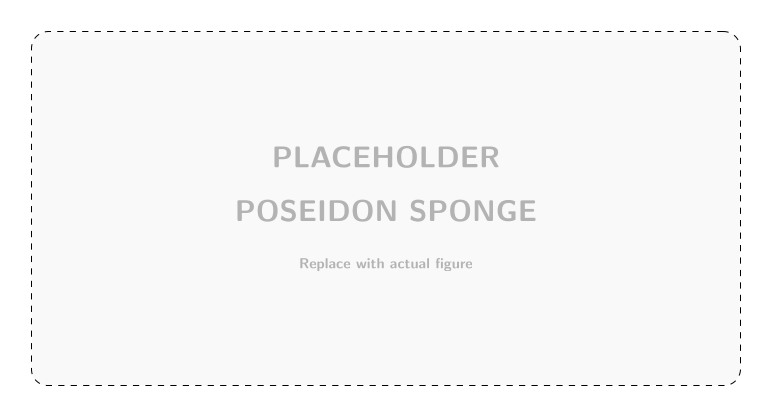
\includegraphics[width=0.85\textwidth]{Images/fig_poseidon_sponge.png}
\caption{Poseidon sponge construction: absorb phase loads inputs into the rate portion; squeeze phase extracts the output hash.}
\label{fig:poseidon-sponge}
\end{figure}

\subsection{Round Function}

Each round of the Poseidon permutation consists of three operations:

\begin{equation}
\text{Round}(S) = \text{MDS} \cdot \text{S-box}(\text{ARK}(S))
\end{equation}

where:
\begin{itemize}
    \item $\text{ARK}(S) = S + C_i$ (Add Round Key: element-wise addition of round constants)
    \item $\text{S-box}(x) = x^5$ (Power map over $\mathbb{F}_r$, chosen for security margin)
    \item $\text{MDS}$ is a Maximum Distance Separable matrix multiplication for diffusion
\end{itemize}

\subsection{Full vs. Partial Rounds}

For security against algebraic attacks while minimizing constraints:
\begin{itemize}
    \item \textbf{Full rounds} ($R_f = 8$): S-box applied to all state elements (diffusion)
    \item \textbf{Partial rounds} ($R_p$): S-box applied to only the first state element (efficiency)
\end{itemize}

For our BN254 instantiation with $t=3$:
\begin{align}
R_f &= 8 \quad \text{(4 before + 4 after partial rounds)} \\
R_p &= 57 \quad \text{(partial rounds)} \\
\text{Total rounds} &= 65
\end{align}

\subsection{Constraint Cost Analysis}

Each full round costs $t$ multiplication gates (one per S-box). Each partial round costs 1 multiplication gate. The MDS multiplication is linear (free in arithmetic circuits). Therefore:

\begin{equation}
\text{Constraints per } \Poseidon_2 \approx R_f \cdot t + R_p = 8 \times 3 + 57 = 81 \text{ multiplication gates}
\end{equation}

In UltraHonk's Plonkish arithmetization, this translates to approximately 300 constraints including the linear operations.

\section{Merkle Tree Membership Proof}

\subsection{Binary Merkle Tree Structure}

\begin{figure}[H]
\centering
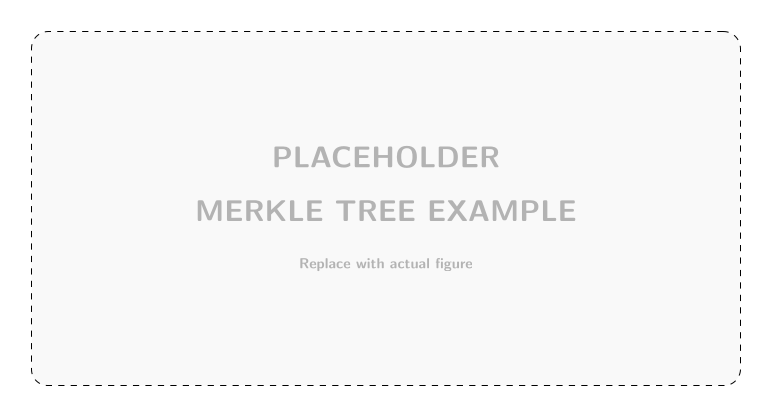
\includegraphics[width=0.85\textwidth]{Images/fig_merkle_tree_example.png}
\caption{Depth-4 Merkle tree example: leaf $l_5$ proves membership by revealing siblings (shaded) along its authentication path.}
\label{fig:merkle-example}
\end{figure}

A binary Merkle tree of depth $d$ stores up to $2^d$ leaves. Each internal node is computed as:
\begin{equation}
\text{node}(i, j) = \Poseidon_2(\text{child\_left}(i, j), \text{child\_right}(i, j))
\end{equation}

\subsection{Authentication Path}

To prove that leaf $l$ is in the tree with root $R$, the prover provides:
\begin{itemize}
    \item The leaf value $l$ (or values that derive it)
    \item The leaf index $i$ (determines left/right placement at each level)
    \item The sibling hash at each level: $\text{siblings}[0], \ldots, \text{siblings}[d-1]$
\end{itemize}

The verifier recomputes the root:
\begin{align}
h_0 &= l \\
h_{k+1} &= \begin{cases}
\Poseidon_2(h_k, \text{siblings}[k]) & \text{if } \text{index\_bits}[k] = 0 \text{ (leaf is left child)} \\
\Poseidon_2(\text{siblings}[k], h_k) & \text{if } \text{index\_bits}[k] = 1 \text{ (leaf is right child)}
\end{cases}
\end{align}

The bit decomposition uses \textbf{little-endian} ordering: bit $k$ of the index determines the direction at tree level $k$ (bottom to top).

\subsection{Variable-Depth Support}

Our tree supports variable depth (up to 16). For a tree with actual depth $d < 16$, the siblings array is padded with zeros for levels $d$ through 15. The circuit uses the \texttt{depth} public input to determine how many levels to traverse.

\section{Complete Noir Circuit Listing}

\begin{lstlisting}[language=Java, caption={Complete Noir ZK voting circuit (main.nr).}, label={lst:circuit}]
use std::hash::poseidon;
use std::hash::poseidon2::Poseidon2;

// Helper: Poseidon hash of single field element
fn poseidon1(input: [Field; 1]) -> Field {
    poseidon::bn254::hash_1(input)
}

// Helper: Poseidon hash of two field elements
fn poseidon2(input: [Field; 2]) -> Field {
    poseidon::bn254::hash_2(input)
}

// Binary Merkle root computation
fn binary_merkle_root<let N: u32>(
    hash_2: fn([Field; 2]) -> Field,
    leaf: Field,
    depth: u32,
    index_bits: [u1; N],
    siblings: [Field; N],
) -> Field {
    let mut current = leaf;
    for i in 0..N {
        if i as u32 < depth {
            let (left, right) = if index_bits[i] == 0 {
                (current, siblings[i])
            } else {
                (siblings[i], current)
            };
            current = hash_2([left, right]);
        }
    }
    current
}

// Main circuit function
fn main(
    nullifier_hash: pub Field,
    root: pub Field,
    vote: pub Field,
    depth: pub u32,
    nullifier: Field,
    secret: Field,
    index: Field,
    siblings: [Field; 16],
) {
    // Constraint 1: Nullifier hash binding
    assert(poseidon1([nullifier]) == nullifier_hash);
    
    // Constraint 2: Commitment derivation
    let commitment = poseidon2([nullifier, secret]);
    
    // Constraint 3: Merkle membership proof
    let index_bits: [u1; 16] = index.to_le_bits();
    let computed_root = binary_merkle_root(
        poseidon2, commitment, depth, index_bits, siblings
    );
    assert(computed_root == root);
    
    // Constraint 4: Vote range check (8-bit)
    let _vote_bits: [u1; 8] = vote.to_le_bits();
}
\end{lstlisting}

\subsection{Line-by-Line Analysis}

\begin{table}[H]
\centering
\caption{Detailed analysis of each circuit constraint.}
\label{tab:constraint-analysis}
\begin{tabular}{|c|p{3cm}|p{4cm}|p{4cm}|}
\hline
\textbf{Line} & \textbf{Operation} & \textbf{Purpose} & \textbf{Security Property} \\
\hline
48 & \texttt{poseidon1([nullifier])} & Compute hash of private nullifier & Binds proof to voter identity \\
\hline
48 & \texttt{== nullifier\_hash} & Assert matches public input & Prevents nullifier substitution \\
\hline
51 & \texttt{poseidon2([null, sec])} & Compute commitment & Links to registered Merkle leaf \\
\hline
54 & \texttt{index.to\_le\_bits()} & Decompose index to bits & Determines path traversal direction \\
\hline
55--57 & \texttt{binary\_merkle\_root} & Compute root from path & Proves set membership \\
\hline
59 & \texttt{== root} & Assert matches chain root & Prevents stale/forged proofs \\
\hline
62 & \texttt{vote.to\_le\_bits()} & 8-bit range check on vote & Prevents overflow attacks \\
\hline
\end{tabular}
\end{table}

\section{Constraint Analysis and Complexity}

\subsection{Constraint Breakdown}

\begin{figure}[H]
\centering
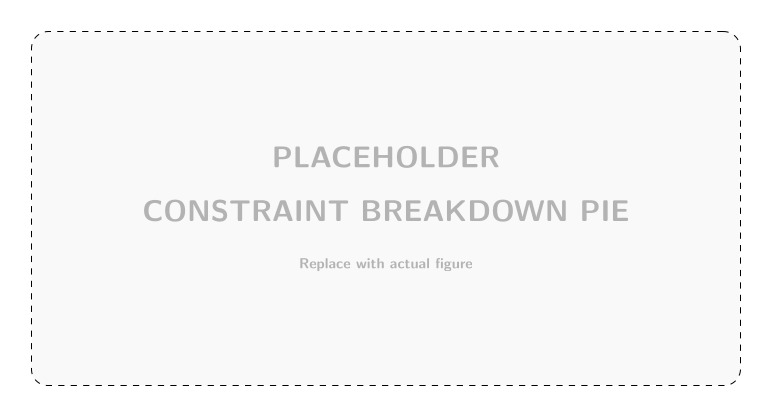
\includegraphics[width=0.85\textwidth]{Images/fig_constraint_breakdown_pie.png}
\caption{Constraint breakdown by operation: Merkle path (16 Poseidon hashes) dominates the circuit size.}
\label{fig:constraint-pie}
\end{figure}

\begin{table}[H]
\centering
\caption{Detailed constraint cost per circuit operation.}
\label{tab:constraint-costs}
\begin{tabular}{|l|r|r|}
\hline
\textbf{Operation} & \textbf{Constraints} & \textbf{Percentage} \\
\hline
Nullifier hash ($\Poseidon_1$) & $\sim$300 & 5.9\% \\
\hline
Commitment ($\Poseidon_2$) & $\sim$300 & 5.9\% \\
\hline
Merkle path (16 $\times$ $\Poseidon_2$) & $\sim$4,800 & 94.1\% \\
\hline
Index bit decomposition & $\sim$16 & 0.3\% \\
\hline
Vote range check & $\sim$8 & 0.2\% \\
\hline
Equality assertions & $\sim$2 & $<$0.1\% \\
\hline
\textbf{Total} & $\sim$5,126 & 100\% \\
\hline
\end{tabular}
\end{table}

\subsection{Asymptotic Complexity}

The circuit complexity scales with tree depth $d$:
\begin{equation}
|\text{Circuit}| = O(d \cdot |\Poseidon_2|) = O(d)
\end{equation}

For our maximum depth of 16, this supports $2^{16} = 65,536$ voters per division. With 160 divisions, the system supports up to $160 \times 65,536 \approx 10.5$ million voters without any circuit modification.

\subsection{Compiled Circuit Size}

After compilation by Nargo to ACIR and then to UltraHonk gates:
\begin{itemize}
    \item \textbf{ACIR opcodes}: $\sim$5,200
    \item \textbf{UltraHonk gates}: $N = 32,768$ ($2^{15}$, next power of 2)
    \item \textbf{LOG\_N}: 15
    \item \textbf{Circuit file size}: $\sim$45 KB (ACIR JSON)
\end{itemize}

\section{UltraHonk Proof System Architecture}

\subsection{Overview}

UltraHonk is a PlonK-variant proof system that eliminates the need for a trusted setup ceremony by using a keccak-based Fiat--Shamir transcript instead of a structured reference string (SRS).

\begin{figure}[H]
\centering
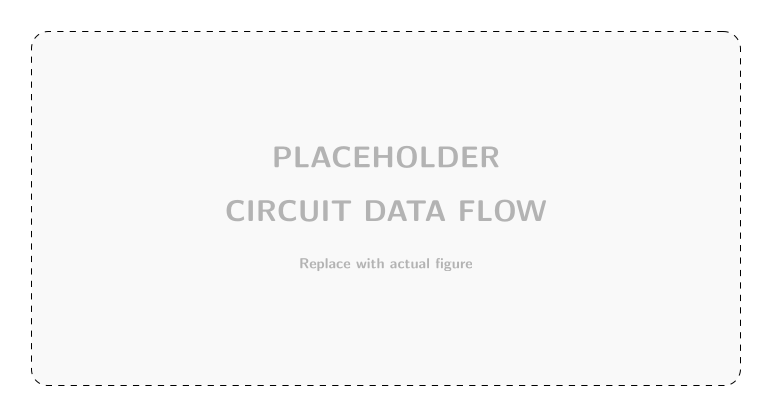
\includegraphics[width=0.85\textwidth]{Images/fig_circuit_data_flow.png}
\caption{UltraHonk proof system data flow: from circuit compilation through ACIR to proof generation and on-chain verification.}
\label{fig:circuit-dataflow}
\end{figure}

\subsection{Arithmetization: Plonkish Constraints}

UltraHonk uses a generalized Plonkish arithmetization supporting:
\begin{itemize}
    \item Standard arithmetic gates: $q_L \cdot a + q_R \cdot b + q_O \cdot c + q_M \cdot (a \cdot b) + q_C = 0$
    \item Custom gates for Poseidon (external and internal rounds)
    \item Lookup tables for range checks
    \item Permutation arguments for wire connections
\end{itemize}

\subsection{Commitment Scheme: KZG on BN254}

Polynomial commitments use the Kate--Zaverucha--Goldberg (KZG) scheme:
\begin{equation}
\text{Commit}(f) = [f(\tau)]_1 = f(\tau) \cdot G_1
\end{equation}

where $\tau$ is the secret evaluation point from the universal SRS. For UltraHonk, the SRS is derived from the Aztec ``ignition'' ceremony (a one-time universal setup supporting circuits up to $2^{28}$ gates).

\subsection{Proof Structure}

An UltraHonk proof consists of:
\begin{enumerate}
    \item Wire polynomial commitments: $[W_1]_1, [W_2]_1, [W_3]_1, [W_4]_1$
    \item Permutation polynomial commitment: $[Z]_1$
    \item Lookup polynomial commitments
    \item Quotient polynomial commitments: $[T_1]_1, [T_2]_1, [T_3]_1, [T_4]_1$
    \item Opening evaluations at challenge point $\zeta$
    \item KZG opening proof: $[W_\zeta]_1, [W_{\zeta\omega}]_1$
\end{enumerate}

Total proof size: approximately 2--4 KB (variable depending on circuit structure).

\section{On-Chain Verifier: HonkVerifier.sol}

\subsection{Auto-Generated Parameters}

The \texttt{HonkVerifier.sol} contract is auto-generated by the Barretenberg compiler from the circuit's verification key:

\begin{lstlisting}[language=Java, caption={HonkVerifier key parameters.}]
uint256 constant N = 32768;           // Circuit size (power of 2)
uint256 constant LOG_N = 15;          // log2(N)
uint256 constant NUMBER_OF_PUBLIC_INPUTS = 4;

// Verification key contains:
// - Selector polynomial commitments (ql, qr, qo, q4, qm, qc, ...)
// - Permutation polynomial commitments (sigma1..4)
// - Identity polynomial commitments (id1..4)
// - Poseidon-specific selectors (qPoseidon2External, qPoseidon2Internal)
\end{lstlisting}

\subsection{Verification Algorithm}

The on-chain verification proceeds in constant time regardless of circuit size:

\begin{algorithm}[H]
\caption{On-Chain Honk Verification (simplified)}
\label{alg:verify}
\begin{algorithmic}[1]
\STATE Parse proof bytes into commitments and evaluations
\STATE Reconstruct Fiat--Shamir challenges from transcript (keccak)
\STATE Compute linearization polynomial evaluation
\STATE Verify KZG opening using BN254 pairing precompile (0x08):
\STATE \quad $e([W_\zeta] + \zeta[W_{\zeta\omega}], [1]_2) \stackrel{?}{=} e([P] + \zeta\omega[W_{\zeta\omega}], [\tau]_2)$
\STATE \textbf{return} pairing check result
\end{algorithmic}
\end{algorithm}

\subsection{Gas Cost}

The verification gas cost is dominated by the BN254 pairing check:
\begin{itemize}
    \item EC additions (precompile 0x06): 150 gas each
    \item EC multiplications (precompile 0x07): 6,000 gas each
    \item Pairing check (precompile 0x08): 45,000 + 34,000 per pair
    \item \textbf{Total verification}: $\sim$280,000 gas
\end{itemize}

\section{Proof Generation Pipeline}

\begin{figure}[H]
\centering
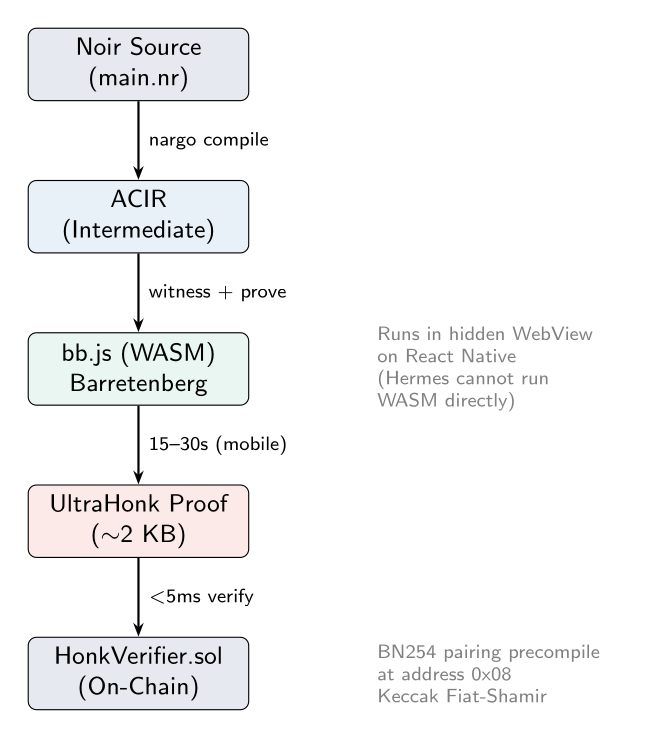
\includegraphics[width=0.85\textwidth]{Images/fig_proof_pipeline.png}
\caption{Complete proof generation pipeline from Noir source code through ACIR compilation to on-chain verification.}
\label{fig:proof-pipeline}
\end{figure}

The end-to-end pipeline consists of five stages:

\begin{enumerate}
    \item \textbf{Circuit Compilation} (build time):
    \begin{itemize}
        \item Nargo compiles \texttt{main.nr} to ACIR (Abstract Circuit Intermediate Representation)
        \item ACIR is a serialized constraint system format
        \item Output: \texttt{circuit.json} ($\sim$45 KB)
    \end{itemize}
    
    \item \textbf{Verification Key Generation} (build time):
    \begin{itemize}
        \item Barretenberg processes ACIR to generate the verification key
        \item Key contains commitments to fixed circuit polynomials
        \item Output: \texttt{HonkVerifier.sol} (auto-generated Solidity contract)
    \end{itemize}
    
    \item \textbf{Witness Computation} (runtime, on device):
    \begin{itemize}
        \item Mobile app constructs the witness from voter secrets and chain state
        \item Witness includes all private inputs satisfying the circuit constraints
    \end{itemize}
    
    \item \textbf{Proof Generation} (runtime, in WebView WASM):
    \begin{itemize}
        \item bb.js WASM module loads ACIR circuit and witness
        \item UltraHonk prover generates the proof (15--30 seconds on mobile)
        \item Output: proof bytes ($\sim$2--4 KB)
    \end{itemize}
    
    \item \textbf{On-Chain Verification} (runtime, EVM):
    \begin{itemize}
        \item Contract calls \texttt{HonkVerifier.verify(proof, publicInputs)}
        \item Verifier uses BN254 precompile for pairing check
        \item Returns boolean: valid or invalid
    \end{itemize}
\end{enumerate}

\section{Security Properties}

\subsection{Computational Soundness}

\begin{theorem}[Soundness]
No probabilistic polynomial-time adversary can produce a valid proof for a false statement (non-member commitment) except with negligible probability:
\begin{equation}
\Pr[\text{Verify}(\pi^*, x) = \text{true} \wedge x \notin L] \leq \text{negl}(\lambda)
\end{equation}
\end{theorem}

This follows from the knowledge soundness of UltraHonk, which is reducible to the algebraic group model (AGM) and the hardness of discrete logarithm on BN254.

\subsection{Zero-Knowledge Property}

\begin{theorem}[Honest-Verifier Zero-Knowledge]
There exists a simulator $S$ that, given only the public inputs $x$, can produce transcripts computationally indistinguishable from real proofs:
\begin{equation}
\{(x, \pi) : \pi \leftarrow P(x, w)\} \approx_c \{(x, \pi^*) : \pi^* \leftarrow S(x)\}
\end{equation}
\end{theorem}

This ensures that the proof reveals nothing about the private witness (nullifier, secret, index, siblings).

\subsection{Double-Vote Prevention}

The nullifier mechanism provides deterministic linkability within a single election:
\begin{equation}
\text{nullifier\_hash} = \Poseidon_1(\text{nullifier}) \quad \text{(deterministic)}
\end{equation}

Two valid proofs from the same voter necessarily produce the same nullifier hash. The contract rejects the second submission, preventing double voting while maintaining anonymity.

\subsection{Front-Running Resistance}

The vote candidate index is a public input bound into the proof:
\begin{equation}
\text{Verify}(\pi, [\text{null\_hash}, \text{root}, v, d]) = \text{true} \implies \text{proof was generated for candidate } v
\end{equation}

An adversary who observes the proof in the mempool cannot extract a valid proof for a different candidate---the proof is cryptographically bound to the specific vote value $v$.

\section{Summary}

This chapter has provided a complete technical analysis of our ZK circuit, from the mathematical foundations of Poseidon and Merkle trees through the Noir implementation to the UltraHonk proof system and on-chain verification. The circuit achieves a constraint count of approximately 5,100 (dominated by 16 Poseidon hashes for the Merkle path), generates proofs in 15--30 seconds on mobile devices, and verifies on-chain in approximately 280,000 gas. The formal security properties (soundness, zero-knowledge, double-vote prevention, and front-running resistance) provide mathematical guarantees suitable for a national-scale election system. Chapter~\ref{ch:contracts} details the smart contracts that consume and enforce these proofs.
